Physical experiments often depend on the
possibility of isolated particles. Examples include experiments where we want to measure the mass or charge of the
trapped particles or collide the particles with
other particles to see what comes out. One way of isolating and
storing the particles, i.e. trapping them, is a Penning trap.

\begin{figure}
  \centering
  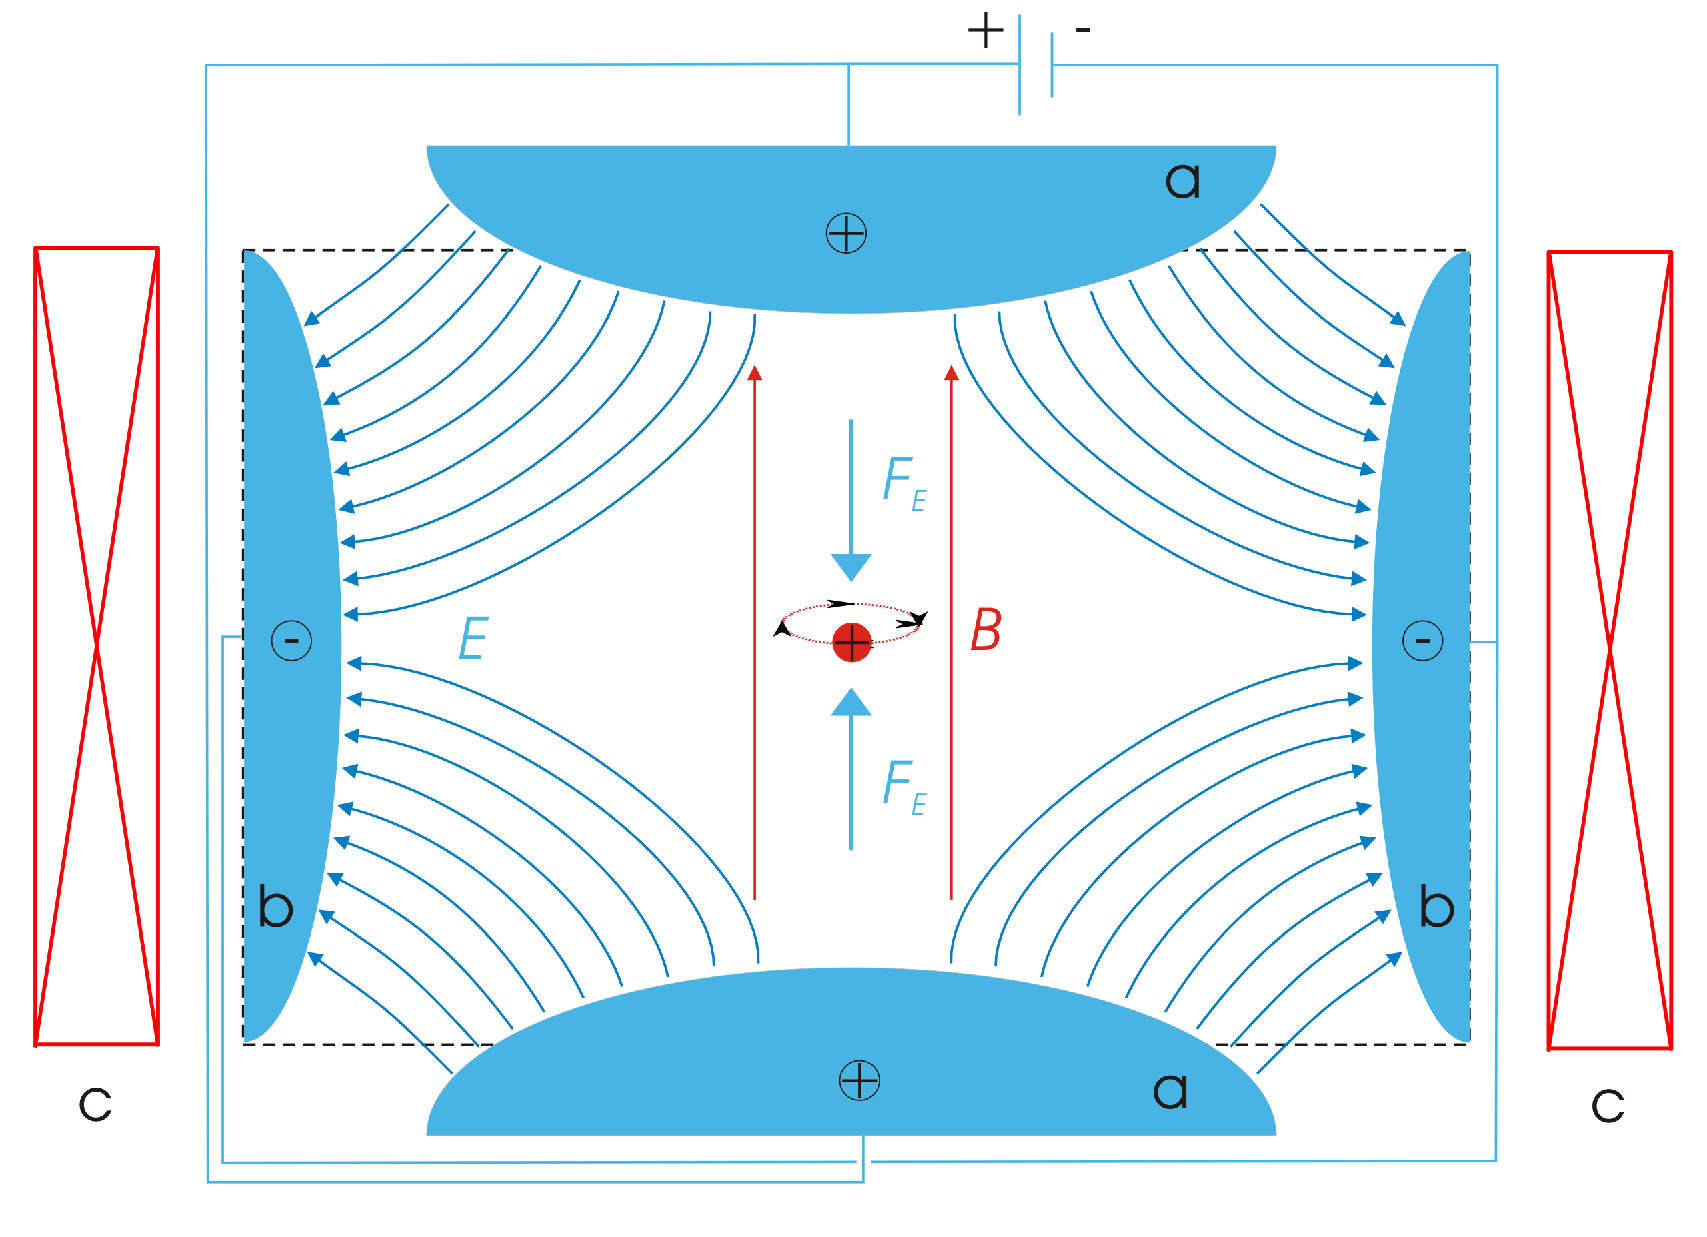
\includegraphics[scale=0.5]{figures/Penning_Trap.pdf}
  \caption{Illustration by Arian Kriesch}% \cite{penning_illustration}}
  \label{fig:penning}
\end{figure}

We want to study the physics of Penning traps using simulations of Ca$^+$-ions.
For many such particles, we will look into the effects of Coulomb interactions on the effectiveness
of the Penning trap. Since the particles are orbiting inside the trap, we can also find resonance
phenomena. The particles might be more susceptible to gaining energy
from the oscillating electric field for specific angular frequencies. We will estimate resonance frequencies for a Penning
trap and see how the Coulomb interactions affect the resonance.

todo: look over this once report we have results, what does the article contain, what do we want to
investigate?
